\section{理论结果}
\label{sec:theory}

我们推导了\labelcref{item:single-neuron-model}中单神经元架构的定位动态的解析模型。
该结果建立了在性质~\labelcref{item:weak-dependence,item:translation-invariance,item:sign-symmetry}下实现定位的充要条件,适用于响应为二值的最简情形,\ie $y = 0,1$。
\cref{sec:experiments} 中展示了,在\labelcref{item:single-neuron-model}中的单神经元架构的定位条件,在经验上同样适用于\labelcref{item:many-neuron-model}中的多神经元架构。
此外,我们利用该模型推导出一个关于定位的负向预测,即尽管这些架构具有非高斯的统计特性——尤其是显著正的峰度——它们在椭圆分布上仍未能学习出局部化的感受野~\parencite[\cf 正峰度作为定位的目标函数或诊断工具,][]{hyvarinen2000independent,ingrosso2022data}。
\subsection{单神经元中定位动力学的分析模型}

先前的研究方法在\labelcref{item:many-neuron-model,item:single-neuron-model}的架构中研究了梯度流,假设预激活$\langle \mathbf{w}, \mathbf{X} \rangle$近似为高斯分布~\parencite{goldt2020modelling,gerace2020generalisation,goldt2022gaussian},但这一假设未能捕捉到通过神经网络传播的高阶统计量,这些统计量促进了定位现象~\cite{ingrosso2022data}。幸运的是,在\labelcref{item:weak-dependence,item:translation-invariance,item:sign-symmetry}中提出的理想化视觉输入设置允许我们进行一些简化。特别地,数据$\mathbf{X}$在\labelcref{item:translation-invariance}下的平移不变性以及\labelcref{item:single-neuron-model}中的架构允许我们使用每个输入维度$X_i$的边际分布,而不是$\mathbf{X}$的联合分布。

我们现在给出允许我们推导单神经元架构中定位动力学的分析模型的简化假设,即对所有$i \in \{1, \dots, N\}$,$\mathbf{X} \mid X_i$的两个假设,以及初始化时满足的权重的温和条件。具体来说,$\sigma_i^y$表示$\Sigma_y$的第$i$行:

\newcounter{assumenumi}
\begin{analysis}{\textbf{解析简化 1--3} (\emph{早期时间,极限动态})}{}
\begin{enumerate}[series=assumenumi]
  \item \label{item:mean-assumption} $\E[\mathbf{X} \mid X_i = x_i, Y = y] = x_i \sigma_i^y$,即条件均值与 $x_i$ 成线性关系。
  \item \label{item:covariance-assumption} $\text{Cov}[\mathbf{X} \mid X_i = x_i, Y = y] = \Sigma_y - \sigma_i^y \sigma_i^{y\top}$,即条件协方差在 $i$ 附近较小,但与 $x_i$ 的确切值无关。
  \item \label{item:lindeberg-condition} Lindeberg 条件对序列 $w_1 X_1, \ldots, w_N X_N \mid X_i = x_i$ 在 $N \to \infty$ 时对所有 $x_i$ 都成立。
\end{enumerate}
\end{analysis}

假设~\labelcref{item:mean-assumption,item:covariance-assumption,item:lindeberg-condition}的动机是,它们复制了边际分布$X_i$(稍后进一步讨论)的峰度,这对于两个重要且不同的极限情形至关重要,其中分别出现和不出现定位现象:当$\mathbf{X}$的支持集中在超立方体的顶点上$\{ \pm 1 \}^N$(对于任意$J$,\texttt{Ising}满足此条件),以及当$\mathbf{X}$是高斯分布时(对于$g \approx 0$的\texttt{NLGP}满足此条件)。

引理~\labelcref{lem:gradient_flow}中的梯度流也依赖于假设~\labelcref{item:lindeberg-condition},即Lindeberg条件对于序列$w_i X_i$成立,这确保了序列中的任何单一项$w_i X_i$不能占主导地位。如果这一条件成立,我们可以得出结论,$\langle \mathbf{w}, \mathbf{X} \rangle \mid X_i$近似为高斯分布。正如我们在\cref{subsec:pf_of_gradient_flow}中讨论的,这几乎总是对$\mathbf{w}$的高斯初始化成立,且对轻微偏离这一初始化的情况也成立,并且满足\textcite{ingrosso2022data}的设置。利用这一事实,我们得到了训练初期梯度流的显式形式,如引理~\labelcref{lem:gradient_flow}所述。

\begin{lemma} \label{lem:gradient_flow}
    在假设~\labelcref{item:mean-assumption,item:covariance-assumption} 下,
    单个ReLU神经元的梯度流在训练初期,假设$y = 0, 1$,使用MSE损失函数时的表达式为
    \begin{equation} \label{eq:gradient_flow_early}
      \frac{2}{\tau} \frac{\mathrm{d}\mathbf{w}}{\mathrm{d}t} = \varphi\left( \frac{\Sigma_1 \mathbf{w}}{\sqrt{\langle \Sigma_1 \mathbf{w}, \mathbf{w} \rangle}} \right) - ( \Sigma_0 + \Sigma_1 ) \mathbf{w} + o_N(1),
    \end{equation}
    其中$o_N(1)$在$N\to\infty$时消失,并且$\varphi : (-1,1) \to \R$ 定义为
    \begin{equation} \label{eq:varphi}
        \varphi(a) = \E_{X_1 \mid Y = 1}\left[ X_1 \operatorname{erf}\left( X_1 \operatorname{alg}^{-1}(a) / \sqrt{2} \right)
        \right]
    \end{equation}
    并且$\operatorname{alg}^{-1}(x) = x/\sqrt{1-x^2}$,是代数sigmoid函数$\operatorname{alg}(x) = x/\sqrt{1+x^2}$的逆函数。
\end{lemma}
引理~\labelcref{lem:gradient_flow}将高阶统计量的研究简化为边际分布$X_1$,由于平移不变性,所有边际分布具有相同的分布,因此我们可以不失一般性地讨论$X_1$。尽管引理~\labelcref{lem:gradient_flow}严格而言只在训练初期成立,且如果$\mathbf{w}$由于违反\labelcref{item:lindeberg-condition}而变得定位,则该引理会失效,但\cref{eq:gradient_flow_early}中的梯度流在足够长的时间内保持有效,足以检测到权重$\mathbf{w}$中的定位现象。特别地,数值积分\cref{eq:gradient_flow_early}会在$t \to \infty$时得到定位的权重$\mathbf{w}$。此外,\cref{eq:gradient_flow_early}中的最终权重峰值的位置与实际观察到的定位峰值位置非常接近;有关这一事实的经验验证,请参见\cref{sec:peak-prediction}。观察到的主要差异是,\cref{eq:gradient_flow_early}中的定位峰值比精确计算的峰值略为平缓;有关实验观测到的定位感受野与理论预测之间的比较,请参见\cref{fig:theory}。
\subsection{涌现局部化的必要和充分条件}
\label{subsec:localization_conditions}

要确定局部化出现的精确阈值,需要求解\cref{eq:gradient_flow_early},但对于一般的非线性微分方程,无法精确求解。\smash{\footnotemark}\footnotetext{
我们在\cref{sec:pde-limit}中讨论了一个面临类似难以处理的偏微分方程极限问题。
}
尽管如此,\cref{eq:gradient_flow_early}的形式表明局部化仅由第一项驱动。
实际上,第二项仅依赖于数据的二阶统计量,因此可以在从诱导局部化的分布变化到不诱导局部化的分布时保持固定。
其次,可以看出,\cref{eq:gradient_flow_early}中的第一项在$\mathbf{w}$缩放时不发生变化,而第二项则有所不同。
因此,\cref{eq:gradient_flow_early}中的第二项用于约束$\mathbf{w}$的\emph{尺度},与局部化不同,而第一项则主要关注$\mathbf{w}$的\emph{形状},因此与局部化相关。
这进一步推动了第一项的关注,因此我们将其称为\emph{放大器},并且它本身依赖于数据分布$p(\mathbf{X})$的性质,
作为研究局部化的重点。

\newcommand{\sampleheight}{42pt}
\newcommand{\covheight}{46pt}
\newcommand{\marginalheight}{50pt}
\setlength{\tabcolsep}{4pt}
\begin{figure}[t]
  \centering
  \hspace{-1.2em}
  \scalebox{0.9}{
  \begin{centering}
    \begin{tabular}{p{51pt}
      @{\hspace{10pt}}m{2pt}l
      @{\hspace{5pt}}l
      @{\hspace{10pt}}m{2pt}l
      @{\hspace{10pt}}m{2pt}l}
        \raisebox{18pt}{\small$\texttt{Ising}$} &
        \raisebox{34pt}{\rotatebox{90}{\tiny input value}} &
        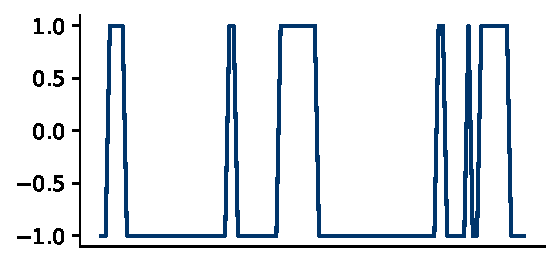
\includegraphics[height=\sampleheight]{figures/task/samples_long/ising.pdf} &
        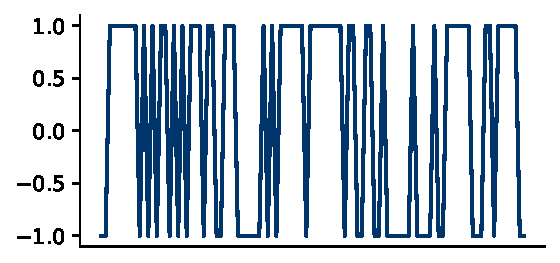
\includegraphics[height=\sampleheight]{figures/task/samples_short/ising.pdf} &
        \raisebox{38pt}{\rotatebox{90}{\tiny input dimension}} &
        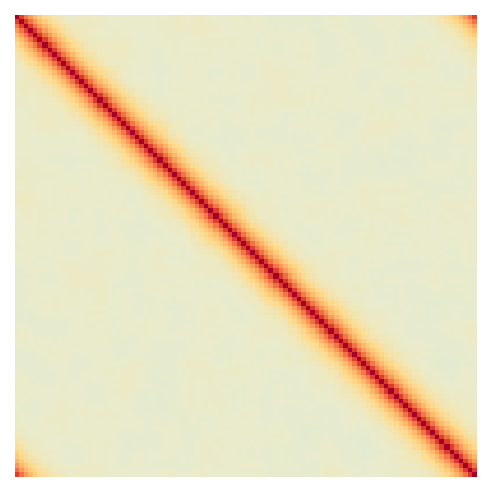
\includegraphics[height=\covheight]{figures/task/cov/ising.pdf} &
        \raisebox{40pt}{\rotatebox{90}{\tiny $p(X_i)$}} &
        \raisebox{-4pt}{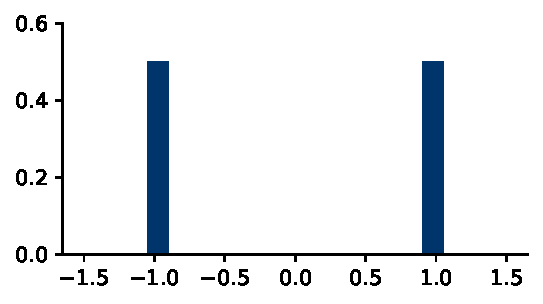
\includegraphics[height=\marginalheight]{figures/task/marginal/ising.pdf}} \\
        \noalign{\vskip -36pt}
        \raisebox{18pt}{\small$\texttt{NLGP}(0.01)$} &
        \raisebox{34pt}{\rotatebox{90}{\tiny input value}} &
        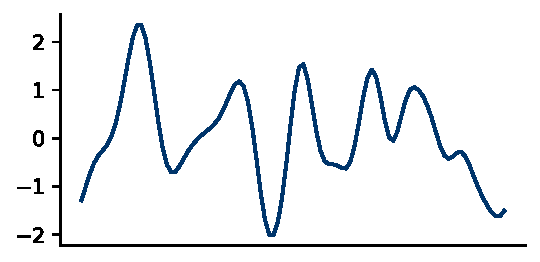
\includegraphics[height=\sampleheight]{figures/task/samples_long/gaussian.pdf} &
        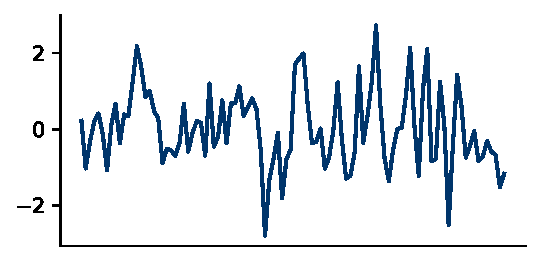
\includegraphics[height=\sampleheight]{figures/task/samples_short/gaussian.pdf} &
        \raisebox{38pt}{\rotatebox{90}{\tiny input dimension}} &
        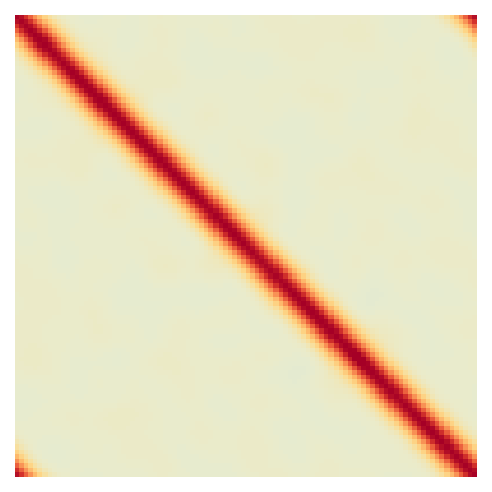
\includegraphics[height=\covheight]{figures/task/cov/gaussian.pdf} &
        \raisebox{40pt}{\rotatebox{90}{\tiny $p(X_i)$}} &
        \raisebox{-4pt}{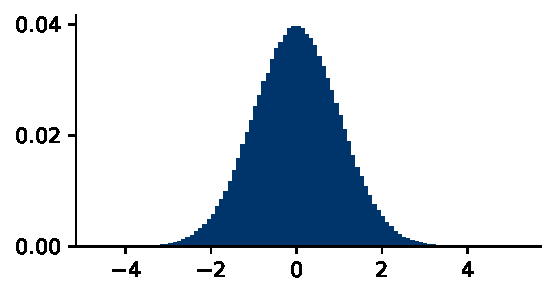
\includegraphics[height=\marginalheight]{figures/task/marginal/gaussian.pdf}} \\
        \noalign{\vskip -36pt}
        \raisebox{18pt}{\small $\texttt{Kur}(5)$} &
        \raisebox{34pt}{\rotatebox{90}{\tiny input value}} &
        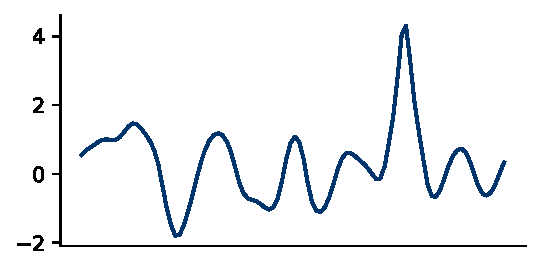
\includegraphics[height=\sampleheight]{figures/task/samples_long/alg5.pdf} &
        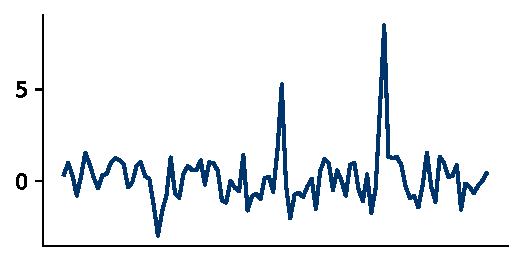
\includegraphics[height=\sampleheight]{figures/task/samples_short/alg5.pdf} &
        \raisebox{38pt}{\rotatebox{90}{\tiny input dimension}} &
        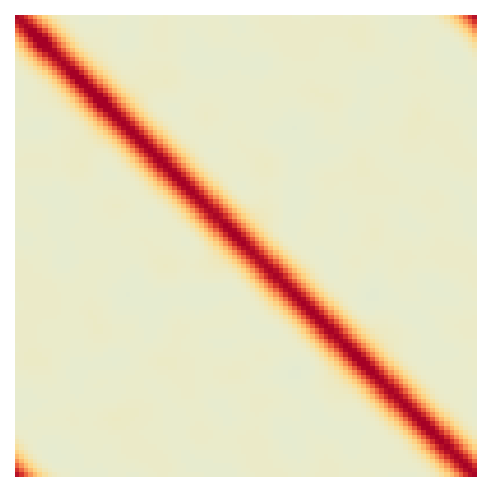
\includegraphics[height=\covheight]{figures/task/cov/alg5.pdf} &
        \raisebox{40pt}{\rotatebox{90}{\tiny $p(X_i)$}} &
        \raisebox{-4pt}{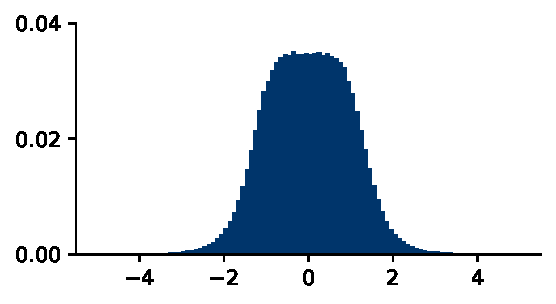
\includegraphics[height=\marginalheight]{figures/task/marginal/alg5.pdf}} \\
        \noalign{\vskip -37pt}
        &&
        \hspace{25pt}\tiny input dimension &
        \hspace{25pt}\tiny input dimension & &
        \hspace{3pt}\tiny input dimension & &
        \hspace{37pt}\tiny input value \\
  \end{tabular}
  \end{centering}
  }
  \caption{
    从左到右:
    长尺度和短尺度样本 $\mathbf{x}$,
    单一尺度的协方差 $\Sigma$,
    以及数据模型的边缘分布 $p(X_i)$,如 \cref{sec:task} 所述:
    Ising 模型(左、右样本分别为 $J=1.2, 0.3$),
    非线性高斯过程~\parencite[NLGP;~][]{ingrosso2022data},
    以及可控峰度模型 \texttt{Kur}
    (左、右样本分别为 $\xi=5, 1$)。
    \emph{
    每个模型生成的样本以零为中心,且其协方差可以被约束为相似,
    但具有不同的高阶统计量,从维度方向的边缘分布中可以看出这一点。
    }
}
  \label{fig:task}
  \vspace{-10pt}
\end{figure}


我们在\cref{sec:varphi-analysis}中对$\varphi$进行了分析,揭示了数据的边际分布在驱动局部化中的作用。
对于每个边际,$\varphi(a) \approx (\sqrt{2/\pi}) a$,当$a \approx 0$时成立。
对于较大的$a$,$\varphi$更强烈地依赖于数据分布,可能是超线性的(亚线性),即大于(小于)$(\sqrt{2/\pi}) a$。
超线性的$\varphi$鼓励在某些邻域中较大的$\mathbf{w}$条目增长得比较小的条目更快,从而产生局部化。
线性和亚线性的$\varphi$则相反,通过抑制$\mathbf{w}$中的邻域,鼓励振荡或平坦的权重。
然而,超线性和亚线性可能并不总是成立,因为$\varphi$可以在其定义域内同时存在(参见\cref{fig:theory},底行,黑线)。
作为一种近似方法,我们考虑了三阶泰勒展开(见\cref{fig:theory}第二列中的红线),这揭示了对于$\sigma^2 = 1$的典型设置,\emph{边际的负过度峰度导致超线性},而\emph{正过度峰度则导致亚线性};
见\cref{sec:varphi-analysis}。
这导致了以下主张,并通过我们在\cref{sec:experiments}中的模拟得到了验证:
\begin{claim} \label{thm:localization}
    对于足够大的 $N$,如果数据 $\mathbf{X} \in \R^N$ 满足条件 \labelcref{item:weak-dependence,item:translation-invariance,item:sign-symmetry} 并且其边际分布具有足够的 \emph{负}过度峰度,则模型~\labelcref{item:single-neuron-model} 将学习到局部化的感受野。
    相反,如果过度峰度足够 \emph{正},则不会。
\end{claim}

作为一个最小的正例,具有最负过度峰度的分布是对称的伯努利分布,峰度值为$-2$。
在我们的设置中,这对应于一个数据向量$\mathbf{X}$,其支持在超立方体的顶点上,$\{ \pm 1 \}^N$。
如上所述,可以从总协方差法则结合符号对称性看出,\labelcref{item:mean-assumption,item:covariance-assumption}完全成立。
请注意,$\varphi$对于所有此类分布是相同的,这使我们得出了\labelcref{thm:localization}的主张,即\emph{任何}满足条件\labelcref{item:weak-dependence,item:translation-invariance,item:sign-symmetry}的分布,其边际最大集中,将在~\labelcref{item:single-neuron-model}中引发局部化的感受野。
值得注意的是,这一主张包括了\textcite{ingrosso2022data}的极限情形,即$\texttt{NLGP}$中的$g\to\infty$。
它还包括了伊辛模型作为另一个例子,验证了对限制玻尔兹曼机的观察 \cite{harsh2020placecell},即伊辛数据在学习模型中引发局部化。
这些主张在\cref{fig:theory}中对单神经元模型进行了验证,并在\cref{sec:experiments}中的多神经元模型中得到了验证。
\subsection{案例研究:椭圆分布未能产生局部化}
\label{sub:elliptical}

如上所述,我们假设弱依赖性(\labelcref{item:weak-dependence})使我们能够专注于边缘分布如何控制局部化。
作为对这种假设的首次调查,我们考虑从椭圆分布中采样的数据 $\mathbf{X}$,其中弱依赖性可能不成立。
我们将椭圆分布的定义~\parencite{frahm2004generalized}专门化到我们的多类标签和符号对称性的设置:
\begin{definition}
    \label{def:elliptical}
    样本 $\mathbf{X} \in \R^N$ 满足 \emph{椭圆分布},如果我们可以写成
    $\mathbf{X} \mid Y = y \overset{(d)}{=} R_y \Lambda_y \mathbf{U}_y$
    其中 $R_y$ 是一个非负随机变量,$\Lambda_y \in \R^{N \times D}$ 满足 $\Lambda_y \Lambda_y^\top = \Sigma_y$,并且 $\mathbf{U}_y$ 与 $R_y$ 独立且在 $D$ 维球面上均匀分布。
\end{definition}

椭圆分布类是广泛的,仅要求密度的等高线是椭圆形的;多元高斯分布和Student-$t$分布就是例子。
因此,它们在非高斯性度量(包括峰度)上可以变化很大,同时保持足够的结构以便于分析。
命题 \labelcref{thm:elliptical} 表明,在单个ReLU神经元模型中,训练椭圆数据会\emph{防止}局部化。
\begin{proposition} \label{thm:elliptical}
  假设数据 $\mathbf{X}$ 是
  符号对称的 (\labelcref{item:sign-symmetry}),
  平移不变的 (\labelcref{item:translation-invariance}),
  并且服从椭圆分布,使得在 \cref{sec:task} 中的任务的均方误差(MSE)始终是有限的。
  如果 $\Sigma_0, \Sigma_1$ 满足它们的第 $i$ 个特征值比率 $\lambda_i(\Sigma_0) / \lambda_i(\Sigma_1)$ 仅在最多两个不同的 $i$ 处取特定值,则 \labelcref{item:single-neuron-model} 中权重的稳态是正弦波,即不局部化。
\end{proposition}

对于数字 $i$ 的条件,使得 $i$-th 特征值的比率相同,限制了在$\mathbf{w}$的稳态中可以非零的傅里叶分量的数量。
尽管这一要求较为晦涩,但在实践中似乎总是成立,因为即使是轻微的长度尺度相关性增加,也能显著改变$\Sigma_y$的谱。

这一命题令人惊讶,因为它揭示了预激活的峰度并不是解释局部化的合适指标。
考虑$N$维Student-$t$分布的例子,具有$\nu$自由度,$t_N(\nu)$。
如果 $\mathbf{X} \sim t_N(\nu)$,则 $\langle w, \mathbf{X} \rangle \sim t_1(\nu)$。
注意,$t_1(\nu)$的峰度是非零的,对于小$\nu$,峰度可以非常大甚至趋于无穷大。
这一预测在\cref{sec:elliptical-experiments}中得到了验证。
这一条件还揭示了并非所有数据中的对称性(这里是椭圆对称性)都会在训练后的模型权重中产生结构,如果局部化被视为比振荡权重更具结构的稀疏性~\parencite[\cf][]{godfrey2023symmetries};实际上,平移对称性(\labelcref{item:translation-invariance})比椭圆对称性在局部化中更为相关。
